% !TEX root = ../dg.tex

\section{Lie Derivatives and Cartan's Magic Formula}

Recall \cref{def:Lie derivative}, the definition of the Lie derivative for vector fields:
\[
	\mathcal{L}_XY := \lim_{t \to 0} \frac{(d\Phi_{-t})_{\Phi_t(p)}Y(\Phi_t(p))-Y(p)}{t},
\]
where $\Phi_t$ is the local flow for $X \in \mathfrak{X}(M)$. We saw in \cref{prop:Lie bracket = Lie derivative} that the Lie derivative is equal to the Lie bracket $[X,Y]$.

The key idea in this derivative was to compare $Y$ at $\Phi_t(p)$ to $Y$ at $p$, and to do so we needed to move $Y(\Phi_t(p))$ from $T_{\Phi_t(p)}M$ to $T_pM$, which we did with the differential of the \emph{negative} flow $d\Phi_{-t}$.

We can use the same idea to get a Lie derivative for differential forms, though we have to be careful about how we move a form $\omega \in \Omega^k(M)$ at a point $\Phi_t(p)$ to $p$: whereas vector fields push forward, differential forms pull back (as we've just seen in \cref{sec:pullbacks}). So rather than pushing forward with $d\Phi_{-t}$, we will pull back by $\Phi_t^\ast$:

\begin{definition}\label{def:Lie derivative of differential form}
	Let $X \in \mathfrak{X}(M)$ and $\omega \in \Omega^k(M)$. Then the \emph{Lie derivative} of $\omega$ with respect to $X$ is defined (at a point $p \in M$) by
	\[
		\left(\mathcal{L}_X\omega\right)_p := \lim_{t \to 0} \frac{\Phi_t^\ast(\omega_{\Phi_t(p)})-\omega_p}{t} = \left. \frac{d}{dt}\right|_{t=0} \Phi_t^\ast(\omega_{\Phi_t(p)}).
	\]
\end{definition}

Even more generally, we can combine pushforwards and pullbacks to get Lie derivatives of arbitrary tensor fields:

\begin{definition}\label{def:Lie derivative of tensor fields}
	Let $X \in \mathfrak{X}(M)$, $a \in \mathcal{T}_r^0(M)$, and $\beta \in \mathcal{T}_0^s(M)$. Then the \emph{Lie derivative} of the $(r,s)$-tensor field $a \otimes \beta$ is defined (at a point $p \in M$) by
	\[
		\left( \mathcal{L}_X a \otimes \beta\right)_p := \left. \frac{d}{dt} \right|_{t=0} \left[ \left(d\Phi_{-t}\right)_{\Phi_t(p)} \left(a _{\Phi_t(p)} \right) \otimes \Phi_t^\ast\left(\beta_{\Phi_t(p)}\right)\right].
	\]
	Extending linearly gives the Lie derivative with respect to $X$ for arbitrary elements of $\mathcal{T}_r^s(M)$.
\end{definition}

\begin{lemma}\label{lem:Lie derivative of function}
	For $f \in C^\infty(M) = \Omega^0(M)$ and $X \in \mathfrak{X}(M)$, 
	\[
		\mathcal{L}_Xf = X(f).
	\]
\end{lemma}

\begin{proof}
	By \cref{def:Lie derivative of differential form} (first equality), \cref{ex:pullbacks of functions are compositions} (second), and \cref{def:tangent vector} (third), 
	\[
		\mathcal{L}_Xf = \left. \frac{d}{dt}\right|_{t=0} \Phi_t^\ast(f) = \left. \frac{d}{dt}\right|_{t=0} f \circ \Phi_t = X(f).
	\]
\end{proof}

\begin{example}
	If $M$ is a manifold and $g$ is a Riemannian metric on $M$, a vector field $X \in \mathfrak{X}(M)$ is called a \emph{Killing field}\footnote{Named after Wilhelm Killing.} if $\mathcal{L}_Xg = 0$. Intuitively, this means that the flow generated by $X$ is an isometry: it preserves distances. If you read about general relativity, you will often see references to Killing fields, which encode the symmetris of spacetime.
	
	Let's compute $\mathcal{L}_X g$ for some vector fields $X$ on $S^2$, where $g$ is the standard Riemannian metric induced by the inner product on $\R^3$. If we work in cylindrical coordinates, we have the local coordinate chart $\phi\from (0,2\pi) \to S^2$ given by
	\[
		\phi(\theta, z) = \left(\sqrt{1-z^2}\cos \theta, \sqrt{1-z^2} \sin \theta, z\right).
	\]
	So then our local coordinate basis $\left\{\frac{\partial}{\partial \theta}, \frac{\partial}{\partial z} \right\}$ at a point $p = \phi(\theta_0,z_0)$ looks like
	\[
		\left. \frac{\partial}{\partial \theta}\right|_p = \left. \frac{d}{dt} \right|_{t=0} \phi(\theta_0+t,z_0) = \left(-\sqrt{1-z_0^2}\sin\theta_0, \sqrt{1-z_0^2}\cos \theta_0,z_0\right)
	\]
	and
	\[
		\left. \frac{\partial}{\partial z}\right|_p = \left. \frac{d}{dt} \right|_{t=0} \phi(\theta_0,z_0+t) = \left(-\frac{z_0 \cos \theta_0}{\sqrt{1-z_0^2}},-\frac{z_0 \sin \theta_0}{\sqrt{1-z_0^2}},1\right).
	\]
	See \cref{fig:dtheta and dz 2} (which is the same as \cref{fig:dtheta and dz}).
	\begin{figure}[htbp]
		\centering
			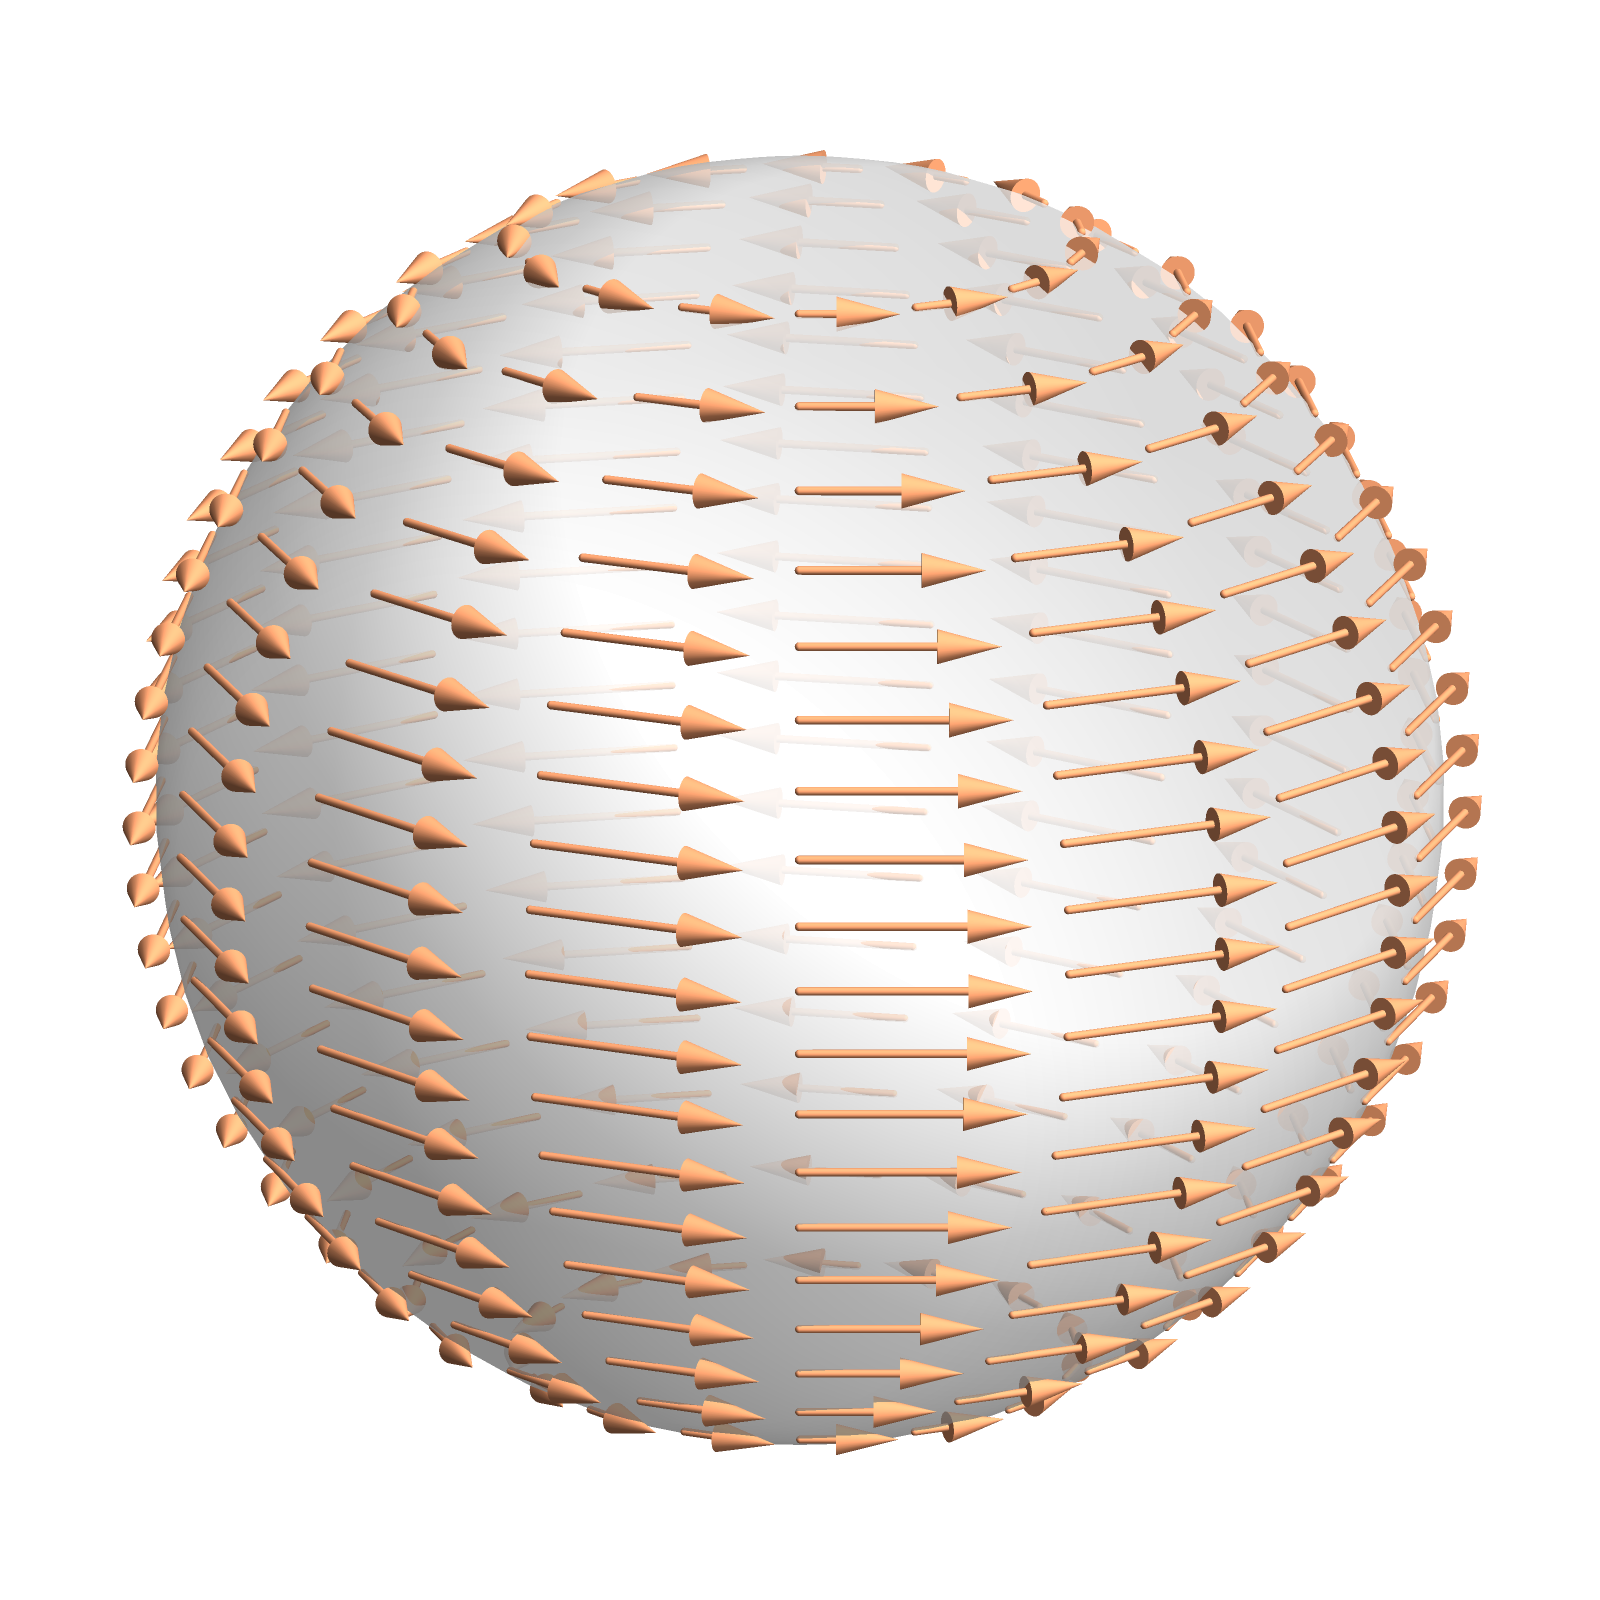
\includegraphics[height=2in]{dtheta} \qquad 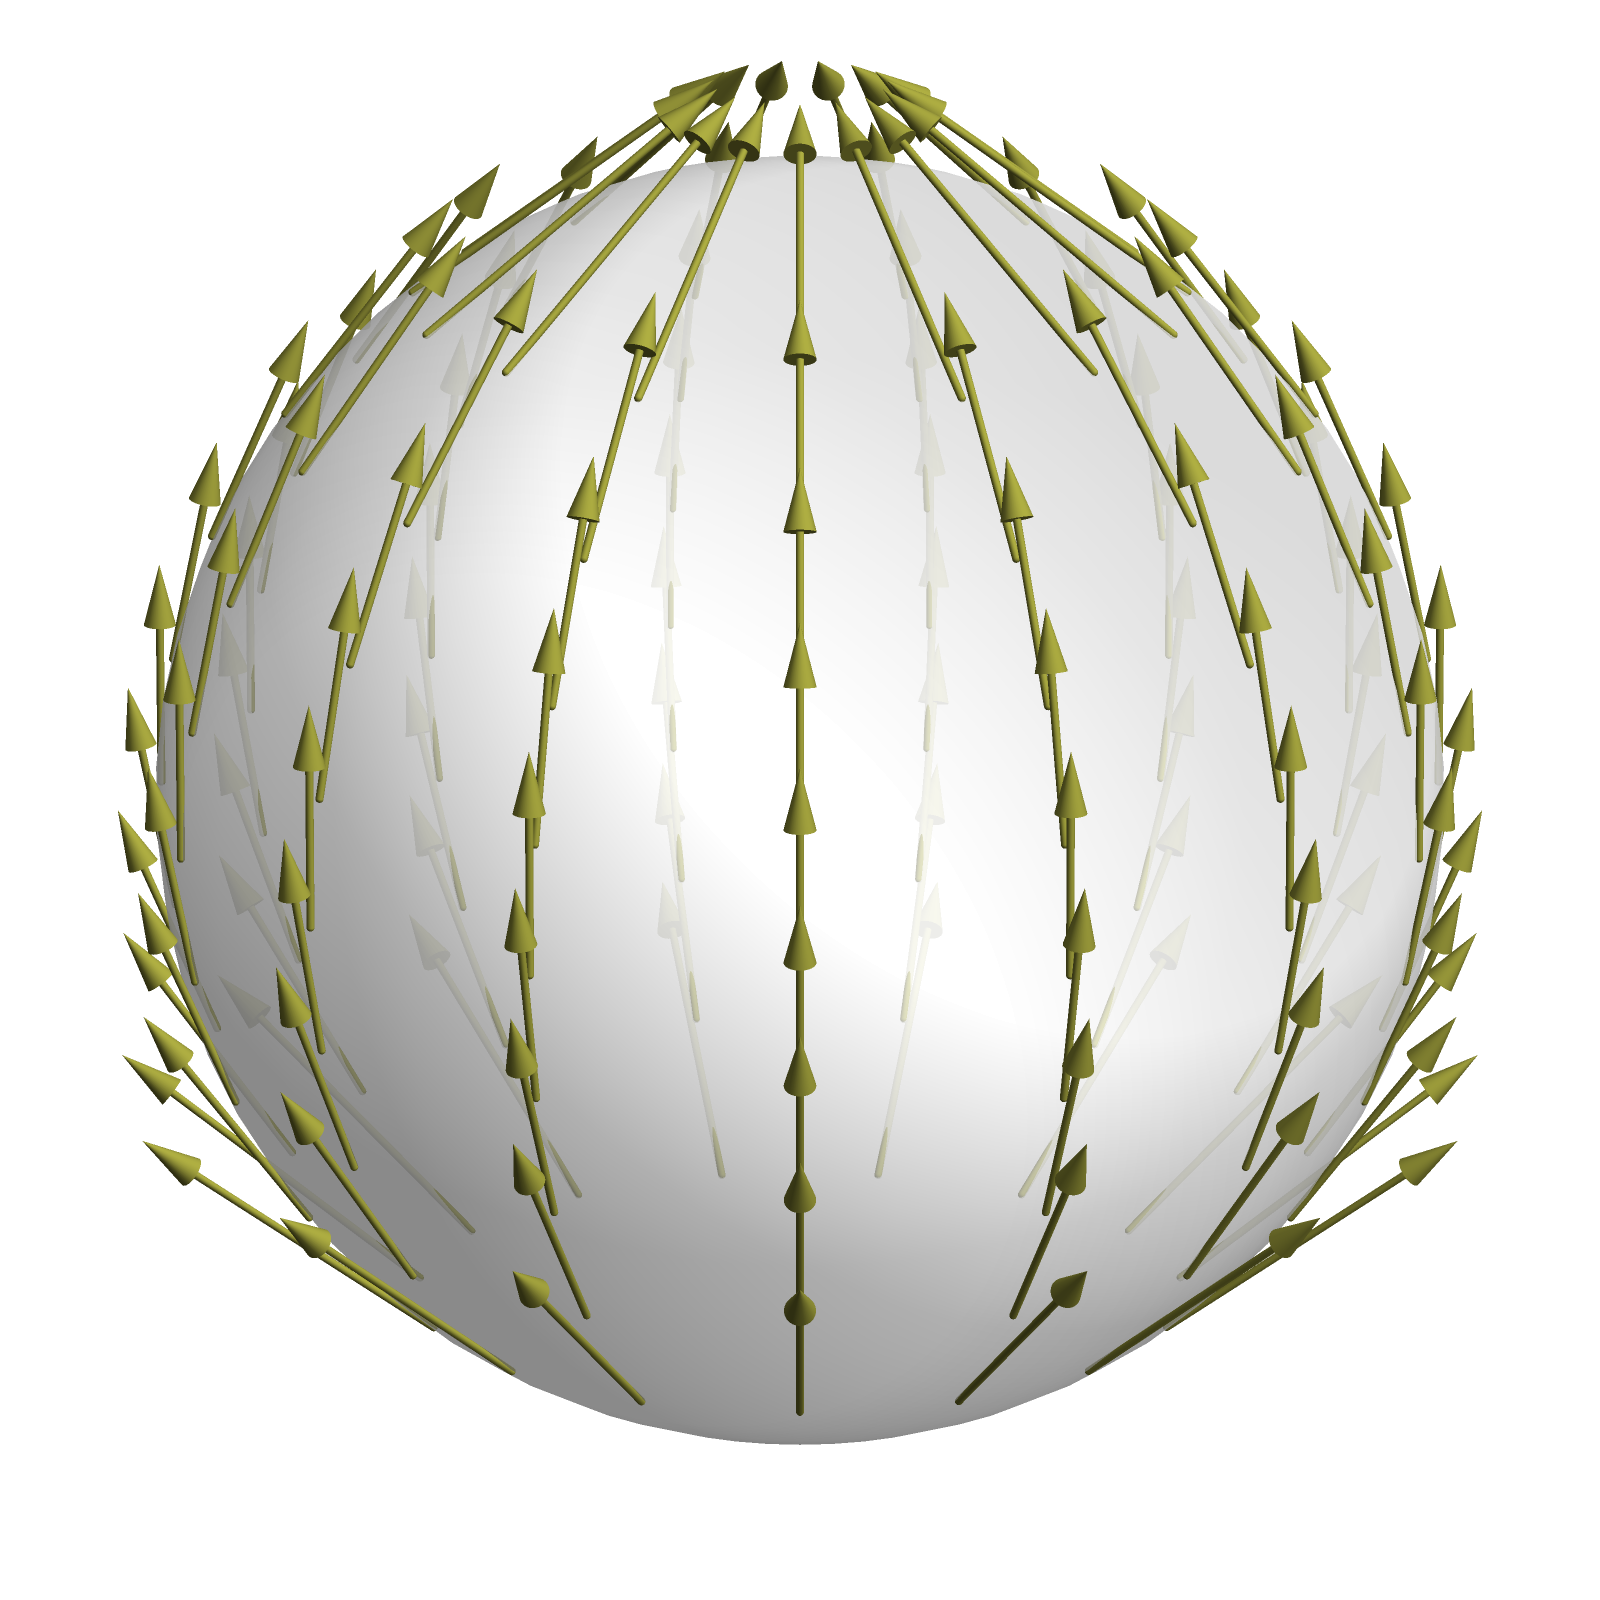
\includegraphics[height=2in]{dz}
		\caption{The vector fields $X = \frac{\partial}{\partial \theta}$ and $Y = \frac{\partial}{\partial z}$ on $S^2$.}
		\alttext{Two computer-generated semi-transparent gray spheres. On the left, a collection of orange arrows or shown on the sphere: the arrows point along circles of latitude: the lengths get shorter as they move away from the equator. On the right, there is a collection of green arrows on the sphere which point towards the north pole. The green arrows get longer as they get further from the equator.}
		\label{fig:dtheta and dz 2}
	\end{figure}
	
	In turn, this implies that the Riemannian metric $g$ is given by
	\begin{align*}
		g_p\left(a \frac{\partial}{\partial \theta} + b \frac{\partial}{\partial z}, c \frac{\partial}{\partial \theta} + d \frac{\partial}{\partial z}\right) & = \left[a\left(-\sqrt{1-z_0^2}\sin\theta_0, \sqrt{1-z_0^2}\cos \theta_0,z_0\right)+ b\left(-\frac{z_0 \cos \theta_0}{\sqrt{1-z_0^2}},-\frac{z_0 \sin \theta_0}{\sqrt{1-z_0^2}},1\right)\right) \\
		& \qquad \cdot \left[c\left(-\sqrt{1-z_0^2}\sin\theta_0, \sqrt{1-z_0^2}\cos \theta_0,z_0\right)+ d\left(-\frac{z_0 \cos \theta_0}{\sqrt{1-z_0^2}},-\frac{z_0 \sin \theta_0}{\sqrt{1-z_0^2}},1\right)\right]  \\
		& = \left(1-z_0^2\right) ac + \frac{1}{1-z_0^2} bd
	\end{align*}
	or, more symbolically,
	\[
		g_{(\theta,z)} = \left(1-z^2\right) d\theta \otimes d\theta + \frac{1}{1-z^2} dz \otimes dz.
	\]
	Notice that this only depends on $z$ and not on $\theta$, so we would expect that flowing by $\frac{\partial}{\partial \theta}$ should preserve this inner product; that is, $\frac{\partial}{\partial \theta}$ should be a Killing field. 
	
	Indeed, the local flow of $\frac{\partial}{\partial \theta}$ is given at a point $p = \phi(\theta_0,z_0)$ by
	\[
		\Phi_t(p) = \phi(\theta_0+t,z) = \left(\sqrt{1-z_0^2}\cos (\theta_0+t), \sqrt{1-z_0^2} \sin (\theta_0+t). z_0\right),
	\]
	Now, writing $\frac{\partial}{\partial \theta} = \alpha'(0)$ where $\alpha(s) = \phi(\theta_0+s,z_0)$, we see that
	\begin{align*}
		(d\Phi_t)_p\left(\left.\frac{\partial}{\partial \theta}\right|_{p}\right) = (d\Phi_t)_p\alpha'(0) & = \left. \frac{d}{ds} \right|_{s=0} (\Phi_t \circ \alpha)(s) \\
		& = \left. \frac{d}{ds} \right|_{s=0} (\Phi_t(\phi(\theta_0+s,z_0)) \\
		& =  \left. \frac{d}{ds} \right|_{s=0} \left(\sqrt{1-z_0^2}\cos (\theta_0+s+t), \sqrt{1-z_0^2} \sin (\theta_0+s+t), z_0\right)  \\
		& = \left(-\sqrt{1-z_0^2}\sin(\theta_0+t),\sqrt{1-z_0^2}\cos(\theta_0+t),0\right) \\
		& = \left. \frac{\partial}{\partial \theta}\right|_{\Phi_t(p)};
	\end{align*}
	i.e., the local flow of $\frac{\partial}{\partial \theta}$ preserves $\frac{\partial}{\partial \theta}$, as you might expect.
	
	On the other hand, $\frac{\partial}{\partial z} = \beta'(0)$ where $\beta(s) = \phi(\theta_0,z_0+s)$, so
	\begin{align*}
		(d\Phi_t)_p\left(\left.\frac{\partial}{\partial z}\right|_{p}\right) = (d\Phi_t)_p\beta'(0) & = \left. \frac{d}{ds} \right|_{s=0} (\Phi_t \circ \beta)(s) \\
		& = \left. \frac{d}{ds} \right|_{s=0} (\Phi_t(\phi(\theta_0,z_0+s)) \\
		& =  \left. \frac{d}{ds} \right|_{s=0} \left(\sqrt{1-(z_0+s)^2}\cos (\theta_0+t), \sqrt{1-(z_0+s)^2} \sin (\theta_0+t), z_0+s\right)  \\
		& = \left(-\frac{z_0 \cos(\theta_0+t)}{\sqrt{1-z_0^2}},-\frac{z_0 \sin(\theta_0+t)}{\sqrt{1-z_0^2}},1\right) \\
		& = \left. \frac{\partial}{\partial z}\right|_{\Phi_t(p)},
	\end{align*}
	so flowing by $\frac{\partial}{\partial \theta}$ also preserves $\frac{\partial}{\partial z}$.

	Therefore, for any $a \left.\frac{\partial}{\partial \theta}\right|_p + b \left.\frac{\partial}{\partial z}\right|_p\in T_pS^2$, we have
	\[
		(d\Phi_t)_p \left(a \left.\frac{\partial}{\partial \theta}\right|_p + b \left.\frac{\partial}{\partial z}\right|_p\right) = a \left.\frac{\partial}{\partial \theta}\right|_{\Phi_t(p)} + b \left.\frac{\partial}{\partial z}\right|_{\Phi_t(p)}.
	\]
	Since $p$ and $\Phi_t(p)$ have the same $z$-coordinate,
	\begin{multline*}
		g_{\Phi_t(p)} \left( a \left.\frac{\partial}{\partial \theta}\right|_{\Phi_t(p)} + b \left.\frac{\partial}{\partial z}\right|_{\Phi_t(p)}, c \left.\frac{\partial}{\partial \theta}\right|_{\Phi_t(p)} + d \left.\frac{\partial}{\partial z}\right|_{\Phi_t(p)}\right) = (1-z_0^2)ac + \frac{1}{1-z_0^2}bd \\
		= g_p\left(a \left.\frac{\partial}{\partial \theta}\right|_p + b \left.\frac{\partial}{\partial z}\right|_p,c \left.\frac{\partial}{\partial \theta}\right|_p + d \left.\frac{\partial}{\partial z}\right|_p\right).
	\end{multline*}
	Hence, for any $u,v \in T_p S^2$
	\[
		(\Phi_t^\ast g_{\Phi_t(p)})(u,v) = g_{\Phi_t(p)}((d\Phi_t)_pu,(d\Phi_t)_pv) = g_p(u,v)
	\]
	is independent of $t$, and we see that
	\[
		(\mathcal{L}_{\frac{\partial}{\partial \theta}} g)_p(u,v) = \left. \frac{d}{dt}\right|_{t=0} (\Phi_t^\ast g_{\Phi_t(p)})(u,v) = 0.
	\]
	Therefore, $\frac{\partial}{\partial \theta}$ is a Killing field on the sphere, which makes sense: the local flow is just rotation around the $z$-axis, which certainly preserves distances.
	
	
	On the other hand, 
	\[
		\Psi_t(p) = \phi(\theta_0,z_0+t) = \left(\sqrt{1-(z_0+t)^2}\cos\theta_0,\sqrt{1-(z_0+t)^2}\sin\theta_0,z_0+t\right)
	\]
	is the local flow of $\frac{\partial}{\partial z}$. So then
	\begin{align*}
		(d\Psi_t)_p\left(\left.\frac{\partial}{\partial \theta}\right|_{p}\right) = (d\Psi_t)_p\alpha'(0) & = \left. \frac{d}{ds} \right|_{s=0} (\Psi_t \circ \alpha)(s) \\
		& = \left. \frac{d}{ds} \right|_{s=0} (\Psi_t(\phi(\theta_0+s,z_0)) \\
		& =  \left. \frac{d}{ds} \right|_{s=0} \left(\sqrt{1-(z_0+t)^2}\cos (\theta_0+s), \sqrt{1-(z_0+t)^2} \sin (\theta_0+s), z_0+t\right)  \\
		& = \left(-\sqrt{1-(z_0+t)^2}\sin\theta_0,\sqrt{1-(z_0+t)^2}\cos\theta_0,0\right) \\
		& = \left. \frac{\partial}{\partial \theta}\right|_{\Psi_t(p)}
	\end{align*}
	and
	\begin{align*}
		(d\Psi_t)_p\left(\left.\frac{\partial}{\partial z}\right|_{p}\right) = (d\Psi_t)_p\beta'(0) & = \left. \frac{d}{ds} \right|_{s=0} (\Psi_t \circ \beta)(s) \\
		& = \left. \frac{d}{ds} \right|_{s=0} (\Psi_t(\phi(\theta_0,z_0+s)) \\
		& =  \left. \frac{d}{ds} \right|_{s=0} \left(\sqrt{1-(z_0+s+t)^2}\cos \theta_0, \sqrt{1-(z_0+s+t)^2} \sin \theta_0, z_0+s+t\right)  \\
		& = \left(-\frac{(z_0+t) \cos\theta_0}{\sqrt{1-(z_0+t)^2}},-\frac{(z_0+t) \sin\theta_0}{\sqrt{1-(z_0+t)^2}},1\right) \\
		& = \left. \frac{\partial}{\partial z}\right|_{\Psi_t(p)},
	\end{align*}
	so flowing by $\frac{\partial}{\partial z}$ also preserves the coordinate vector fields, but the coordinate vector fields do not have constant length on $S^2$. 
	
	We see that 
	\begin{multline*}
		(\Psi_t^\ast g_{\Psi_t(p)})\left(a \left.\frac{\partial}{\partial \theta}\right|_p + b \left.\frac{\partial}{\partial z}\right|_p, c \left.\frac{\partial}{\partial \theta}\right|_p + d \left.\frac{\partial}{\partial z}\right|_p\right) =  g_{\Psi_t(p)}\left(a \left.\frac{\partial}{\partial \theta}\right|_{\Psi_t(p)} + b \left.\frac{\partial}{\partial z}\right|_{\Psi_t(p)}, c \left.\frac{\partial}{\partial \theta}\right|_{\Psi_t(p)} + d \left.\frac{\partial}{\partial z}\right|_{\Psi_t(p)}\right)  \\
		= (1-(z_0+t)^2)ac + \frac{1}{1-(z_0+t)^2}bd,
	\end{multline*}
	and hence
	\begin{multline*}
		(\mathcal{L}_{\frac{\partial}{\partial z}} g)_p\left(\left.\frac{\partial}{\partial \theta}\right|_p,\left.\frac{\partial}{\partial \theta}\right|_p\right) = \left. \frac{d}{dt}\right|_{t=0} (\Psi_t^\ast g_{\Psi_t(p)})\left(\left.\frac{\partial}{\partial \theta}\right|_p,\left.\frac{\partial}{\partial \theta}\right|_p\right) = \left. \frac{d}{dt}\right|_{t=0} \left[(1-(z_0+t)^2)ac + \frac{1}{1-(z_0+t)^2}bd\right] \\
		= -2z_0 ac + \frac{2z_0}{(1-z_0^2)^2}bd;
	\end{multline*}
	that is,
	\[
		\mathcal{L}_{\frac{\partial}{\partial z}} g = -2z\, d\theta \otimes d\theta + \frac{2z}{(1-z^2)^2}dz \otimes dz,
	\]
	which is no longer positive-definite (and hence not a Riemannian metric), but is still a symmetric $(0,2)$-tensor field on $S^2$ which captures how $g$ changes as we flow in the $\frac{\partial}{\partial z}$ direction.
\end{example}

One of the most important formulas in differential geometry is:
\begin{theorem}[Cartan's Magic Formula]\label{thm:cartan}
	If $\omega \in \Omega^k(M)$ and $X \in \mathfrak{X}(M)$, then
	\[
		\mathcal{L}_X \omega = \iota_X d\omega + d \iota_X \omega.
	\]
\end{theorem}
Here $\iota_X$ is the \emph{contraction operator} (or \emph{interior product}) defined as follows: for $\omega \in \Omega^k(M)$ and $X \in \mathfrak{X}(M)$, $\iota_X\omega$ is the $(k-1)$-form defined by
\[
	(\iota_X\omega)_p(v_1, \dots , v_{k-1}) = \omega_p(X(p),v_1, \dots , v_{k-1})
\]
for any $v_1, \dots , v_{k-1} \in T_pM$. This is sometimes also denoted by $X \lrcorner \omega$. This is an antiderivation of degree $-1$.

The reason Cartan's magic formula is so important is that it is one of the most useful tools out there for computing exterior derivatives.

\begin{example}\label{ex:cartan and S^3}
	Remember \cref{sec:S^3 example}, where we computed Lie brackets on $S^3$. As a reminder, we had mutually perpendicular vector fields $X,Y,Z \in \mathfrak{X}(S^3)$ defined by
	\[
		X(p) = pi, \qquad Y(p) = pj, \qquad Z(p) = pk
	\]
	for all $p \in S^3$ thought of as unit quaternions, and showed that
	\[
		[X,Y]=2Z, \qquad [Y,Z] = 2X, \qquad [Z,X] = 2Y.
	\]
	Let $\alpha, \beta, \gamma$ be the dual 1-forms; that is, $\alpha(X) = 1$, $\alpha(Y) = 0 = \alpha(Z)$ and similarly for $\beta$ and $\gamma$. Then, using Cartan's magic formula,
	\[
		d\alpha(Y,Z) = (\iota_Y d\alpha)(Z) = (\mathcal{L}_Y\alpha)(Z) - d(\iota_Y\alpha)(Z) = (\mathcal{L}_Y\alpha)(Z) -d(\alpha(Y))(Z) = (\mathcal{L}_Y\alpha)(Z)
	\]
	since $\alpha(Y) = 0$.
	
	The Lie derivative turns out to be a derivation, so it obeys a Leibniz rule:
	\[
		\mathcal{L}_U(\omega(Y_1, \dots , Y_k)) = (\mathcal{L}_U\omega)(Y_1, \dots , Y_k) + \sum_{j=1}^k \omega(Y_1, \dots , \mathcal{L}_U Y_j, \dots , Y_k).
	\]
	In particular,
	\[
		0 = \mathcal{L}_Y(0) = \mathcal{L}_Y(\alpha(Z)) = (\mathcal{L}_Y \alpha)(Z) + \alpha(\mathcal{L}_YZ) = (\mathcal{L}_Y \alpha)(Z) + \alpha([Y,Z]) = (\mathcal{L}_Y \alpha)(Z) + \alpha(2X) = (\mathcal{L}_Y \alpha)(Z) + 2,
	\]
	so we conclude that
	\[
		d\alpha(Y,Z) = (\mathcal{L}_Y\alpha)(Z) = -2.
	\]
	By analogous calculations, we can show that $d\alpha(X,Y) = 0 = d\alpha(Z,X)$, so we conclude that
	\[
		d\alpha = -2 \beta \wedge \gamma,
	\] 
	and similarly one can show that $d\beta = 2\gamma \wedge \alpha$ and $d\gamma = -2 \alpha \wedge \beta$.
	
	This implies, in particular, that $\alpha \wedge d\alpha = -2 \alpha \wedge \beta \wedge \gamma$ is never zero, so $\alpha$ is an example of what is called a \emph{contact form} on $S^3$.
\end{example}

Notice, in particular, that we never had to work in local coordinates in \cref{ex:cartan and S^3}, which is one of the great virtues of Cartan's magic formula: it is one of the few tools that allows one to compute without using coordinates.

Hopefully this gives you some reason to believe that Cartan's magic formula is useful, so let's try to prove it:

\begin{proof}[Proof of \cref{thm:cartan}]
	If $u \in \Omega^0(M) = C^\infty(M)$, then $\mathcal{L}_Xu = X(u)$ by \cref{lem:Lie derivative of function} and
	\[
		\iota_X du + d\iota_Xu = du(X) + 0 = du(X) = X(u) = \mathcal{L}_Xu ,
	\]
	so the formula holds for 0-forms.
	
	Now consider a 1-form $\omega$ which is the differential of a 0-form: $\omega = du$. If $Y \in \mathfrak{X}(M)$, then, by \cref{def:Lie derivative of differential form},
	\[
		(\mathcal{L}_X\omega)_p(Y) = (\mathcal{L}_xdu)_p(Y) = \left. \frac{d}{dt} \right|_{t=0} \Phi_t^\ast(du_{\Phi_t(p)})(Y) = (\mathcal{L}_xdu)_p(Y) = \left. \frac{d}{dt} \right|_{t=0} du_{\Phi_t(p)}((d\Phi_t)_p(Y))
	\]
	using the definition of pullback (\cref{def:pullback}). In turn, the chain rule tells us that the right hand side is equal to
	\[
		\left. \frac{d}{dt} \right|_{t=0} d(u \circ\Phi_t)_p(Y) = \left. \frac{d}{dt} \right|_{t=0} Y(u \circ\Phi_t)(p)
	\]
	by \cref{lem:vector fields and differentials}. Since $Y$ is independent of $t$, the (1-dimensional) chain rule tell us that this is equal to
	\[
		Y \left( \left. \frac{d(u \circ \Phi_t)}{dt} \right|_{t=0}\right)(p) = Y(X(u))(p).
	\]
	
	So we have shown that $(\mathcal{L}_X\omega)_p(Y) = Y(X(u))(p)$.
	
	On the other hand, $\iota_X d\omega = \iota_X d(du) = 0$ and
	\[
		d(\iota_X\omega)(Y) = d(\iota_X du)(Y) = d(du(X))(Y) = d(X(U))(Y) = Y(X(U)) = (\mathcal{L}_X\omega)_p(Y)
	\]
	by repeatedly using \cref{lem:vector fields and differentials}. Hence, the formula holds for differentials.
	
	Finally, then, if $\omega \in \Omega^k(M)$ and we write $\omega = \sum_I a_I dx_I$ in local coordinates, then
	\begin{equation}\label{eq:cartan in local coords1}
		\mathcal{L}_X\omega = \sum_I \left[ (\mathcal{L}_X a_I)dx_I + a_I \mathcal{L}_X(dx_I)\right].
	\end{equation}
	The $k=0$ argument above implies that 
	\begin{equation}\label{eq:carten in local coords2}
		\mathcal{L}_X a_I = (\iota_X d + d \iota_X)a_I.
	\end{equation} 
	
	On the other hand, again using the fact that the Lie derivative is a derivation, we have
	\begin{multline*}
		\mathcal{L}_X (dx_{i_1} \wedge \dots \wedge dx_{i_k}) = \sum_{j=1}^k dx_{i_1} \wedge \dots \wedge \mathcal{L}_X dx_{i_j}  \wedge \dots \wedge  dx_{i_k} = \sum_{j=1}^k dx_{i_1} \wedge \dots \wedge (\iota_X d + d \iota_X) dx_{i_j}  \wedge \dots \wedge dx_{i_k} \\
		= (\iota_X d + d \iota_X)(dx_{i_1} \wedge \dots \wedge dx_{i_k})
	\end{multline*}
	since each $dx_{i_j}$ is a differential.
	
	Combining this with \eqref{eq:cartan in local coords1} and \eqref{eq:carten in local coords2} implies that 
	\[
		\mathcal{L}_X\omega = \sum_I \left[ ((\iota_X d + d \iota_X) a_I)dx_I + a_I (\iota_X d + d \iota_X)(dx_I)\right] = (\iota_X d + d \iota_X)\sum_I a_I dx_I = (\iota_X d + d \iota_X)\omega,
	\]
	as desired.
\end{proof}